\subsection{Test 1:}

The first test consist in encode an empty file using the program provided in the folder {\bfseries Encoder}, as we said, if the file it's empty, the program will take the string {\itshape "This is a test for Huffman's algorithm"}. As we can see in Figure 4.1.0, the {\itshape Original.txt} file it's empty, so, we will run the program and see what's in {\itshape Frequency.txt} and {\itshape Codification.txt} files ( Figures 4.1.1 and 4.1.2 ). \hfill \break

\begin{figure}[H]
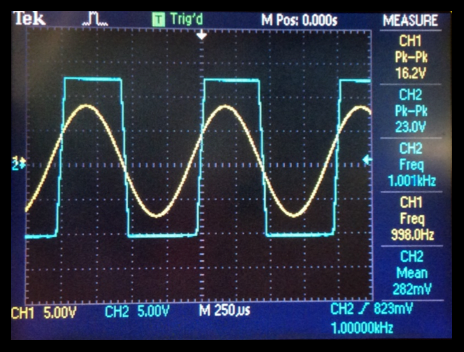
\includegraphics[height = 2cm, width = 16.5cm]{o1.png}
\centering \linebreak \linebreak Figure 4.1.0: Empty Original.txt file.
\end{figure} \hfill \break

\begin{multicols}{2}
\begin{figure}[H]
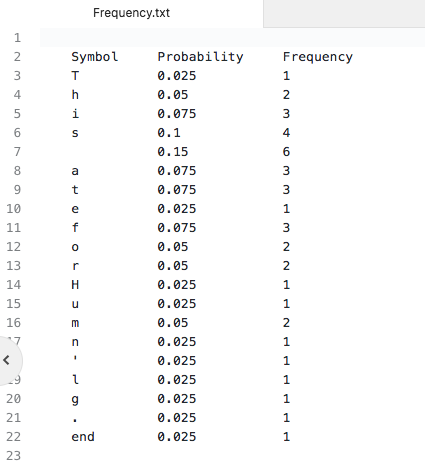
\includegraphics[height = 8cm, width = 6cm]{f1.png}
\centering \linebreak \linebreak Figure 4.1.1: Frequency.txt file for the string {\itshape "This is a test for Huffman's algorithm"}.
\end{figure} \hfill \break

\begin{figure}[H]
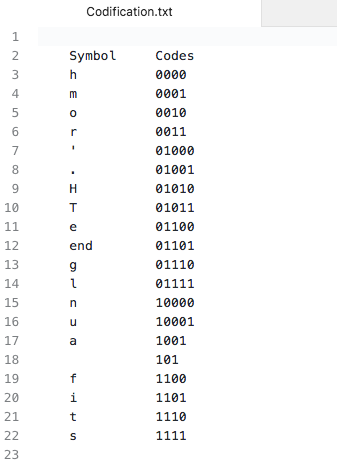
\includegraphics[height = 8cm, width = 6cm]{c1.png}
\centering \linebreak \linebreak Figure 4.1.2: Codification of each {\itshape symbol} for the string {\itshape "This is a test for Huffman's algorithm"}.
\end{figure} \hfill \break
\end{multicols} 

The output text or {\itshape binary-string} generated by the encoder program it's presented in Figure 4.1.3, as we have previously mentioned, we import the python module {\bfseries pickle} that server for binary inputs and outputs. \hfill \break

\begin{figure}[H]
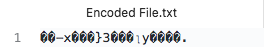
\includegraphics[height = 2cm, width = 8cm]{b1.png}
\centering \linebreak \linebreak Figure 4.1.3: Encoded File.txt 
\end{figure} \hfill \break

For decoding we run the program provided in the folder {\bfseries Decoder} that will take as parameters what ever it is in the file presented in Figure 4.1.3 and the dictionary of codes. Finally, after executing the decoding process, the program will generate a file named {\itshape Decoded File.txt}, as you can imagine, will store the decoded text. Figure 4.1.4 shows this output. \hfill \break

\begin{figure}[H]
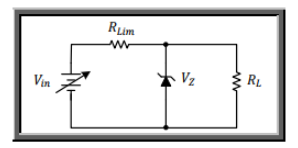
\includegraphics[height = 2cm, width = 16.5cm]{d1.png}
\centering \linebreak \linebreak Figure 4.1.4: Decoded File.txt
\end{figure} \hfill \break

Finally, to see if the encoder program actually compress the size of the string {\itshape "This is a test for Huffman's algorithm} with the help of the {\itshape system information} we visualize that the size of the decoded file it's bigger ( Figure 4.1.5 ) than the encoded one ( Figure 4.1.6 ). \hfill \break

\begin{multicols}{2}
\begin{figure}[H]
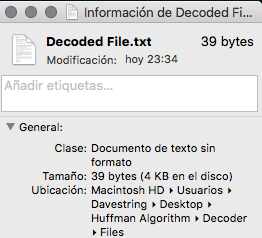
\includegraphics[height = 6cm, width = 6cm]{sd1.png}
\centering \linebreak \linebreak Figure 4.1.5: Decoded file size.
\end{figure} \hfill \break

\begin{figure}[H]
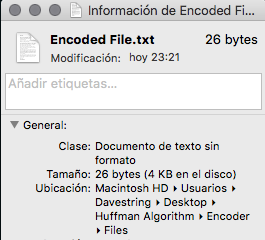
\includegraphics[height = 6cm, width = 6cm]{se1.png}
\centering \linebreak \linebreak Figure 4.1.6: Encoded file size.
\end{figure} \hfill \break
\end{multicols} 

As we can see the Decoded file has a size of 39 bytes in comparison with the Encoded one that has a size of 26 bytes.

\pagebreak